\documentclass{../gdutthesis}

\gdutsetup{
  style/cover         = {false},
}

\usepackage{glossaries}
\renewcommand{\loadglsentries}[1]{}
\usepackage{zhlipsum, pgffor}

% % 文本页面中可以被顶部浮动占用的最大比例,默认值 0.7
% \renewcommand*{\topfraction}{0.9}

% % 文本页面中可被底部浮动占用的最大比例,默认值 0.3
% \renewcommand*{\bottomfraction}{0.9}

% % 必须由文本占用的文本页的最小比例,默认值 0.2
% \renewcommand*{\textfraction}{0.1}

% % 在生成“浮动页面”之前必须被浮动体占用的页面的最小比例,默认值 0.5
% \renewcommand*{\floatpagefraction}{0.9}

\begin{document}
\foreach \i in {2,4,6,8}
  {
    \zhlipsum[1-2]
    \begin{figure}
      \centering
      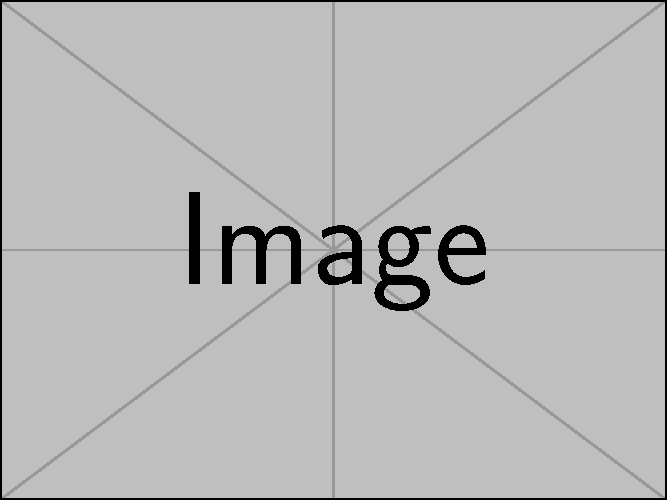
\includegraphics[width=\textwidth,height=0.\i\textheight]{example-image.pdf}
    \end{figure}
    \zhlipsum[3]
    \clearpage
  }
\end{document}